\section{Implementation}\label{sec:implementation}

The introduced quantum circuit preparation schemes have been implemented in the python package \qcreason{}, which architecture is sketched in \figref{fig:qcreasonArchitecture}.
\begin{figure}[t]
    \begin{center}
        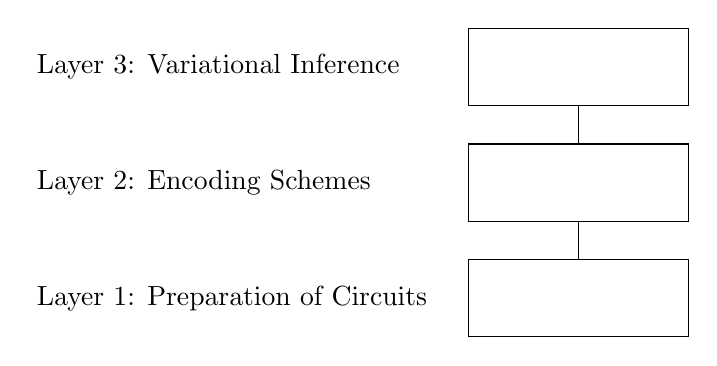
\begin{tikzpicture}[scale=0.35,yscale=0.7]
    \draw (-10,10) rectangle (-2,14);
    \node [anchor=center] at (-6,12) {\spreasoning{}};
    \node [anchor=west] at (-26,12) {Layer 3: Variational Inference};

    \draw (-6,10) -- (-6,8);
    \draw (-10,4) rectangle (-2,8);
    \node [anchor=center] at (-6,6) {\sprepresentation{}};
    \node [anchor=west] at (-26,6) {Layer 2: Encoding Schemes};

    \draw (-6,4) -- (-6,2);
    \draw (-10,-2) rectangle (-2,2);
    \node [anchor=center] at (-6,0) {\spengine{}};
    \node [anchor=west] at (-26,0) {Layer 1: Preparation of Circuits};
\end{tikzpicture}
    \end{center}
    \caption{Architecture of the \textcolor{\pythonblue}{\qcreason{}} package.
    The \spinference{} sub-package receives inference tasks from \tnreason{} and calls \sppreparation{} and \spsimulation{} for corresponding circuit preparation and simulation.}
    \label{fig:qcreasonArchitecture}
\end{figure}

\subsection{Quantum Circuits}

Quantum Circuits are stored as lists of dictionaries, where each dictionary represents a quantum gate application.
% Unitaries
We specify the unitaries by strings accessible via the key \stringof{unitary}, as listed in the following table:
\begin{center}
    \begin{tabular}{|c|c|c|c|}
        \hline
        \textbf{Unitary}         & \textbf{String Representation} & \textbf{Parameters} & \textbf{Tensor Notation}                                                   \\
        \hline
        Hadamard                 & \stringof{H}                   &                     & $\hgateat{\catvariableof{\insymbol},\catvariableof{\outsymbol}}$           \\
        Pauli-X                  & \stringof{X}                   &                     & $\paulixat{\cavariable{\insymbol},\cavariable{\outsymbol}}$              \\
        %Multiple controlled $X$  & \stringof{MCX}                 &                     &                                                                            \\
        Rotation around $Y$-axis & \stringof{RY}                 & Angle $\alpha$      & $\yrotationofat{\alpha}{\cavariable{\insymbol},\cavariable{\outsymbol}}$ \\
        \hline
    \end{tabular}
\end{center}


% Controlled
The control in controlled operations is specified by a dictionary accessible via the key \stringof{control}.
It contains as keys the control qubits and their control states as values (i.e. the state in which the unitary is applied).

% Parameters
Further parameters such as angles are added in another dictionary, accessible via the key \stringof{parameters}.

% Example
For example a hadamard gate on qubit \stringof{blue} and a multiple controlled rotation around the $Y$-axis on qubit \stringof{ancilla\_c1} controlled by qubits \stringof{red} and \stringof{blue} in state $(0,1)$ with an angle is represented as:
\begin{minted}{python}
[{'unitary': 'H',
    'target': ['blue']},
{'unitary': 'MCRY',
    'target': ['ancilla_c1'],
    'control': {'red': 1, 'blue': 0},
    'parameters': {'angle': np.float64(0.6121442808462428)}}]
\end{minted}
Note that we omit the notation of incoming and outgoing variables.

\subsection{Generic Contraction}

So far, the generic contraction routine consists in activation circuits preparing for each tensor an ancilla variable, and post-selecting the measurements where the ancilla variable is $1$.
The resulting tensor of the contraction is a $\mathrm{PandasCore}$ storing the post-selected measurement results in a dataframe.